% Tanenbaum 2003 - Section 4.3 Ethernet
\chapter{Ethernet}
\label{chap:ethernet}

We have now finished our general discussion of channel allocation
protocols in the abstract, so it is time to see how these principles
apply to real systems, in particular, LANs. As discussed in
\protect\hyperlink{0130661023_ch01lev1sec5.htmlux5cux23ch01lev2sec23}{Sec.
1.5.3}, the IEEE has standardized a number of local area networks and
metropolitan area networks under the name of IEEE 802. A few have
survived but many have not, as we saw in
\protect\hyperlink{0130661023_ch01lev1sec6.htmlux5cux23ch01fig38}{Fig.
1-38}. Some people who believe in reincarnation think that Charles
Darwin came back as a member of the IEEE Standards Association to weed
out the unfit. The most important of the survivors are 802.3 (Ethernet)
and 802.11 (wireless LAN). With 802.15 (Bluetooth) and 802.16 (wireless
MAN), it is too early to tell. Please consult the 5th edition of this
book to find out. Both 802.3 and 802.11 have different physical layers
and different MAC sublayers but converge on the same logical link
control sublayer (defined in 802.2), so they have the same interface to
the network layer.

We introduced Ethernet in
\protect\hyperlink{0130661023_ch01lev1sec5.htmlux5cux23ch01lev2sec23}{Sec.
1.5.3} and will not repeat that material here. Instead we will focus on
the technical details of Ethernet, the protocols, and recent
developments in high-speed (gigabit) Ethernet. Since Ethernet and IEEE
802.3 are identical except for two minor differences that we will
discuss shortly, many people use the terms ``Ethernet'' and ``IEEE
802.3'' interchangeably, and we will do so, too. For more information
about Ethernet, see (Breyer and Riley, 1999 ; Seifert, 1998; and
Spurgeon, 2000).

\section{Ethernet cabling}

Since the name ``Ethernet'' refers to the cable (the ether), let us start our discussion there.
Four types of cabling are commonly used, as shown in \cref{fig:common-ethernet-cabling}.


\begin{table}
   \centering
   %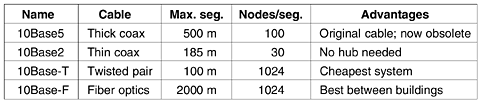
\includegraphics[width=\textwidth]{images/04fig13.png}
   \begin{tabular}{rlrrl}
   \textit{name}     & cable         & max. seg. & nodes/seg. & advantages                   \\[.75ex]
   \textit{10Base5}  & thick coax    &    500\,m &        100 & original cable; now obsolete \\
   \textit{10Base2}  & thin coax     &    185\,m &         30 & no hub needed                \\
   \textit{10Base-T} & twisted pair  &    100\,m &       1024 & cheapest system              \\
   \textit{10Base-F} & fiber optics  &   2000\,m &       1024 & best between buildings       \\
   \end{tabular}
   \caption{The most common kinds of Ethernet cabling.}
   \label{fig:common-ethernet-cabling}
\end{table}


Historically, \emph{10Base5} cabling, popularly called \emph{thick Ethernet}, came first.
It resembles a yellow garden hose, with markings every 2.5~meters to show where the taps go.
(The 802.3 standard does not actually \emph{require} the cable to be yellow, but it does \emph{suggest} it.)
Connections to it are generally made using \emph{vampire taps}, in which a pin is \emph{very} carefully forced halfway into the coaxial cable's core.
The notation 10Base5 means that it operates at 10\,Mbps, uses baseband signaling, and can support segments of up to 500~meters.
The first number is the speed
in Mbps. Then comes the word ``Base'' (or sometimes ``BASE'') to
indicate baseband transmission. There used to be a broadband variant,
10Broad36, but it never caught on in the marketplace and has since
vanished. Finally, if the medium is coax, its length is given rounded to
units of 100\,m after ``Base.''

Historically, the second cable type was \emph{10Base2}, or \emph{thin Ethernet,}
which, in contrast to the garden-hose-like thick Ethernet, bends easily.
Connections to it are made using industry-standard BNC connectors to
form T junctions, rather than using vampire taps. BNC connectors are
easier to use and more reliable. Thin Ethernet is much cheaper and
easier to install, but it can run for only 185~meters per segment, each of which can handle only 30~machines.

Detecting cable breaks, excessive length, bad taps, or loose connectors
can be a major problem with both media. For this reason, techniques have
been developed to track them down. Basically, a pulse of known shape is
injected into the cable. If the pulse hits an obstacle or the end of the
cable, an echo will be generated and sent back. By carefully timing the
interval between sending the pulse and receiving the echo, it is
possible to localize the origin of the echo. This technique is called
\emph{time domain reflectometry}.

The problems associated with finding cable breaks drove systems toward a
different kind of wiring pattern, in which all stations have a cable
running to a central {hub} in which they are all connected electrically
(as if they were soldered together). Usually, these wires are telephone
company twisted pairs, since most office buildings are already wired
this way, and normally plenty of spare pairs are available. This scheme
is called {10Base-T}. Hubs do not buffer incoming traffic. We will
discuss an improved version of this idea (switches), which do buffer
incoming traffic later in this chapter.

These three wiring schemes are illustrated in \cref{fig:three-ethernet-cabling}.
For 10Base5, a {transceiver} is clamped securely around the cable
so that its tap makes contact with the inner core. The transceiver
contains the electronics that handle carrier detection and collision
detection. When a collision is detected, the transceiver also puts a
special invalid signal on the cable to ensure that all other
transceivers also realize that a collision has occurred.


\begin{figure}
   \centering
   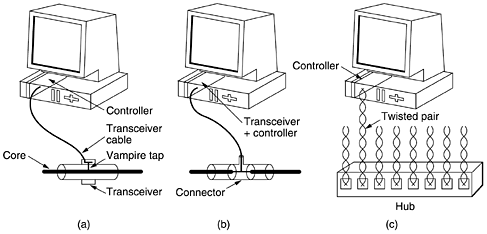
\includegraphics[width=.7\textwidth]{images/04fig14.png}
   \caption{Three kinds of Ethernet cabling. (a) 10Base5. (b) 10Base2. (c) 10Base-T.}
   \label{fig:three-ethernet-cabling}
\end{figure}


With 10Base5, a {transceiver cable} or {drop cable} connects the
transceiver to an interface board in the computer. The transceiver cable
may be up to 50 meters long and contains five individually shielded
twisted pairs. Two of the pairs are for data in and data out,
respectively. Two more are for control signals in and out. The fifth
pair, which is not always used, allows the computer to power the
transceiver electronics. Some transceivers allow up to eight nearby
computers to be attached to them, to reduce the number of transceivers
needed.

The transceiver cable terminates on an interface board inside the
computer. The interface board contains a controller chip that transmits
frames to, and receives frames from, the transceiver. The controller is
responsible for assembling the data into the proper frame format, as
well as computing checksums on outgoing frames and verifying them on
incoming frames. Some controller chips also manage a pool of buffers for
incoming frames, a queue of buffers to be transmitted, direct memory
transfers with the host computers, and other aspects of network
management.

With 10Base2, the connection to the cable is just a passive BNC
T-junction connector. The transceiver electronics are on the controller
board, and each station always has its own transceiver.

With 10Base-T, there is no shared cable at all, just the hub (a box full
of electronics) to which each station is connected by a dedicated (i.e.,
not shared) cable. Adding or removing a station is simpler in this
configuration, and cable breaks can be detected easily. The disadvantage
of 10Base-T is that the maximum cable run from the hub is only 100
meters, maybe 200 meters if very high quality category 5 twisted pairs
are used. Nevertheless, 10Base-T quickly became dominant due to its use
of existing wiring and the ease of maintenance that it offers. A faster
version of 10Base-T (100Base-T) will be discussed later in this chapter.

A fourth cabling option for Ethernet is {10Base-F}, which uses fiber
optics. This alternative is expensive due to the cost of the connectors
and terminators, but it has excellent noise immunity and is the method
of choice when running between buildings or widely-separated hubs. Runs
of up to km are allowed. It also offers good security since wiretapping
fiber is much more difficult than wiretapping copper wire.

\protect\hyperlink{0130661023_ch04lev1sec3.htmlux5cux23ch04fig15}{Figure
4-15} shows different ways of wiring a building. In
\protect\hyperlink{0130661023_ch04lev1sec3.htmlux5cux23ch04fig15}{Fig.
4-15(a)}, a single cable is snaked from room to room, with each station
tapping into it at the nearest point. In
\protect\hyperlink{0130661023_ch04lev1sec3.htmlux5cux23ch04fig15}{Fig.
4-15(b)}, a vertical spine runs from the basement to the roof, with
horizontal cables on each floor connected to the spine by special
amplifiers (repeaters). In some buildings, the horizontal cables are
thin and the backbone is thick. The most general topology is the tree,
as in
\protect\hyperlink{0130661023_ch04lev1sec3.htmlux5cux23ch04fig15}{Fig.
4-15(c)}, because a network with two paths between some pairs of
stations would suffer from interference between the two signals.

\subparagraph[Figure 4-15. Cable topologies. (a) Linear. (b) Spine. (c)
Tree. (d)
Segmented.]{\texorpdfstring{\protect\hypertarget{0130661023_ch04lev1sec3.htmlux5cux23ch04fig15}{}{}Figure
4-15. Cable topologies. (a) Linear. (b) Spine. (c) Tree. (d)
Segmented.}{Figure 4-15. Cable topologies. (a) Linear. (b) Spine. (c) Tree. (d) Segmented.}}

%\includegraphics{04fig15.gif}

Each version of Ethernet has a maximum cable length per segment. To
allow larger networks, multiple cables can be connected by {repeaters},
as shown in
\protect\hyperlink{0130661023_ch04lev1sec3.htmlux5cux23ch04fig15}{Fig.
4-15(d)}. A repeater is a physical layer device. It receives, amplifies
(regenerates), and retransmits signals in both directions. As far as the
software is concerned, a series of cable segments connected by repeaters
is no different from a single cable (except for some delay introduced by
the repeaters). A system may contain multiple cable segments and
multiple repeaters, but no two transceivers may be more than 2.5 km
apart and no path between any two transceivers may traverse more than
four repeaters.

\protect\hypertarget{0130661023_ch04lev1sec3.htmlux5cux23ch04lev2sec10}{}{}

\section{Manchester Encoding}

None of the versions of Ethernet uses straight binary encoding with 0
volts for a 0 bit and 5 volts for a 1 bit because it leads to
ambiguities. If one station sends the bit string 0001000, others might
falsely interpret it as 10000000 or 01000000 because they cannot tell
the difference between an idle sender (0 volts) and a 0 bit (0 volts).
This problem can be solved by using +1 volts for a 1 and -1 volts for a
0, but there is still the problem of a receiver sampling the signal at a
slightly different frequency than the sender used to generate it.
Different clock speeds can cause the receiver and sender to get out of
synchronization about where the bit boundaries are, especially after a
long run of consecutive 0s or a long run of consecutive 1s.

What is needed is a way for receivers to unambiguously determine the
start, end, or middle of each bit without reference to an external
clock. Two such approaches are called {Manchester encoding} and
{differential Manchester encoding}. With Manchester encoding, each bit
period is divided into two equal intervals. A binary 1 bit is sent by
having the voltage set high during the first interval and low in the
second one. A binary 0 is just the reverse: first low and then high.
This scheme ensures that every bit period has a transition in the
middle, making it easy for the receiver to synchronize with the sender.
A disadvantage of Manchester encoding is that it requires twice as much
bandwidth as straight binary encoding because the pulses are half the
width. For example, to send data at 10 Mbps, the signal has to change 20
million times/sec. Manchester encoding is shown in
\protect\hyperlink{0130661023_ch04lev1sec3.htmlux5cux23ch04fig16}{Fig.
4-16(b)}.

\subparagraph[Figure 4-16. (a) Binary encoding. (b) Manchester encoding.
(c) Differential Manchester
encoding.]{\texorpdfstring{\protect\hypertarget{0130661023_ch04lev1sec3.htmlux5cux23ch04fig16}{}{}Figure
4-16. (a) Binary encoding. (b) Manchester encoding. (c) Differential
Manchester
encoding.}{Figure 4-16. (a) Binary encoding. (b) Manchester encoding. (c) Differential Manchester encoding.}}

%\includegraphics{04fig16.gif}

Differential Manchester encoding, shown in
\protect\hyperlink{0130661023_ch04lev1sec3.htmlux5cux23ch04fig16}{Fig.
4-16(c)}, is a variation of basic Manchester encoding. In it, a 1 bit is
indicated by the absence of a transition at the start of the interval. A
0 bit is indicated by the presence of a transition at the start of the
interval. In both cases, there is a transition in the middle as well.
The differential scheme requires more complex equipment but offers
better noise immunity. All Ethernet systems use Manchester encoding due
to its simplicity. The high signal is + 0.85 volts and the low signal is
- 0.85 volts, giving a DC value of 0 volts. Ethernet does not use
differential Manchester encoding, but other LANs (e.g., the 802.5 token
ring) do use it.

\protect\hypertarget{0130661023_ch04lev1sec3.htmlux5cux23ch04lev2sec11}{}{}

\section{The Ethernet MAC sublayer protocol}

The original DIX (DEC, Intel, Xerox) frame structure is shown in
\protect\hyperlink{0130661023_ch04lev1sec3.htmlux5cux23ch04fig17}{Fig.
4-17(a)}. Each frame starts with a {Preamble} of 8 bytes, each
containing the bit pattern 10101010. The Manchester encoding of this
pattern produces a 10-MHz square wave for 6.4 µsec to allow the
receiver's clock to synchronize with the sender's. They are required to
stay synchronized for the rest of the frame, using the Manchester
encoding to keep track of the bit boundaries.

\subparagraph[Figure 4-17. Frame formats. (a) DIX Ethernet. (b) IEEE
802.3.]{\texorpdfstring{\protect\hypertarget{0130661023_ch04lev1sec3.htmlux5cux23ch04fig17}{}{}Figure
4-17. Frame formats. (a) DIX Ethernet. (b) IEEE
802.3.}{Figure 4-17. Frame formats. (a) DIX Ethernet. (b) IEEE 802.3.}}

%\includegraphics{04fig17.gif}

The frame contains two addresses, one for the destination and one for
the source. The standard allows 2-byte and 6-byte addresses, but the
parameters defined for the 10-Mbps baseband standard use only the 6-byte
addresses. The high-order bit of the destination address is a 0 for
ordinary addresses and 1 for group addresses. Group addresses allow
multiple stations to listen to a single address. When a frame is sent to
a group address, all the stations in the group receive it. Sending to a
group of stations is called {multicast}. The address consisting of all 1
bits is reserved for {broadcast}. A frame containing all 1s in the
destination field is accepted by all stations on the network. The
difference between multicast and broadcast is important enough to
warrant repeating. A multicast frame is sent to a selected group of
stations on the Ethernet; a broadcast frame is sent to all stations on
the Ethernet. Multicast is more selective, but involves group
management. Broadcasting is coarser but does not require any group
management.

Another interesting feature of the addressing is the use of bit 46
(adjacent to the high-order bit) to distinguish local from global
addresses. Local addresses are assigned by each network administrator
and have no significance outside the local network. Global addresses, in
contrast, are assigned centrally by IEEE to ensure that no two stations
anywhere in the world have the same global address. With 48 - 2 = 46
bits available, there are about 7 x 10\textsuperscript{13} global
addresses. The idea is that any station can uniquely address any other
station by just giving the right 48-bit number. It is up to the network
layer to figure out how to locate the destination.

Next comes the {Type} field, which tells the receiver what to do with
the frame. Multiple network-layer protocols may be in use at the same
time on the same machine, so when an Ethernet frame arrives, the kernel
has to know which one to hand the frame to. The {Type} field specifies
which process to give the frame to.

Next come the data, up to 1500 bytes. This limit was chosen somewhat
arbitrarily at the time the DIX standard was cast in stone, mostly based
on the fact that a transceiver needs enough RAM to hold an entire frame
and RAM was expensive in 1978. A larger upper limit would have meant
more RAM, hence a more expensive transceiver.

In addition to there being a maximum frame length, there is also a
minimum frame length. While a data field of 0 bytes is sometimes useful,
it causes a problem. When a transceiver detects a collision, it
truncates the current frame, which means that stray bits and pieces of
frames appear on the cable all the time. To make it easier to
distinguish valid frames from garbage, Ethernet requires that valid
frames must be at least 64 bytes long, from destination address to
checksum, including both. If the data portion of a frame is less than 46
bytes, the {Pad} field is used to fill out the frame to the minimum
size.

Another (and more important) reason for having a minimum length frame is
to prevent a station from completing the transmission of a short frame
before the first bit has even reached the far end of the cable, where it
may collide with another frame. This problem is illustrated in
\protect\hyperlink{0130661023_ch04lev1sec3.htmlux5cux23ch04fig18}{Fig.
4-18}. At time 0, station {A}, at one end of the network, sends off a
frame. Let us call the propagation time for this frame to reach the
other end {t}. Just before the frame gets to the other end (i.e., at
time {t}-{e}), the most distant station, {B}, starts transmitting. When
{B} detects that it is receiving more power than it is putting out, it
knows that a collision has occurred, so it aborts its transmission and
generates a 48-bit noise burst to warn all other stations. In other
words, it jams the ether to make sure the sender does not miss the
collision. At about time 2{t}, the sender sees the noise burst and
aborts its transmission, too. It then waits a random time before trying
again.

\subparagraph[Figure 4-18. Collision detection can take as long as
2{t}.]{\texorpdfstring{\protect\hypertarget{0130661023_ch04lev1sec3.htmlux5cux23ch04fig18}{}{}Figure
4-18. Collision detection can take as long as
2{t}.}{Figure 4-18. Collision detection can take as long as 2t.}}

%\includegraphics{04fig18.gif}

If a station tries to transmit a very short frame, it is conceivable
that a collision occurs, but the transmission completes before the noise
burst gets back at 2{t}. The sender will then incorrectly conclude that
the frame was successfully sent. To prevent this situation from
occurring, all frames must take more than 2{t} to send so that the
transmission is still taking place when the noise burst gets back to the
sender. For a 10-Mbps LAN with a maximum length of 2500 meters and four
repeaters (from the 802.3 specification), the round-trip time (including
time to propagate through the four repeaters) has been determined to be
nearly 50 µsec in the worst case, including the time to pass through the
repeaters, which is most certainly not zero. Therefore, the minimum
frame must take at least this long to transmit. At 10 Mbps, a bit takes
100 nsec, so 500 bits is the smallest frame that is guaranteed to work.
To add some margin of safety, this number was rounded up to 512 bits or
64 bytes. Frames with fewer than 64 bytes are padded out to 64 bytes
with the {Pad} field.

As the network speed goes up, the minimum frame length must go up or the
maximum cable length must come down, proportionally. For a 2500-meter
LAN operating at 1 Gbps, the minimum frame size would have to be 6400
bytes. Alternatively, the minimum frame size could be 640 bytes and the
maximum distance between any two stations 250 meters. These restrictions
are becoming increasingly painful as we move toward multigigabit
networks.

The final Ethernet field is the {Checksum}. It is effectively a 32-bit
hash code of the data. If some data bits are erroneously received (due
to noise on the cable), the checksum will almost certainly be wrong and
the error will be detected. The checksum algorithm is a cyclic
redundancy check (CRC) of the kind discussed in
\protect\hyperlink{0130661023_ch03.htmlux5cux23ch03}{Chap. 3}. It just
does error detection, not forward error correction.

When IEEE standardized Ethernet, the committee made two changes to the
DIX format, as shown in
\protect\hyperlink{0130661023_ch04lev1sec3.htmlux5cux23ch04fig17}{Fig.
4-17(b)}. The first one was to reduce the preamble to 7 bytes and use
the last byte for a {Start of Frame} delimiter, for compatibility with
802.4 and 802.5. The second one was to change the {Type} field into a
{Length} field. Of course, now there was no way for the receiver to
figure out what to do with an incoming frame, but that problem was
handled by the addition of a small header to the data portion itself to
provide this information. We will discuss the format of the data portion
when we come to logical link control later in this chapter.

Unfortunately, by the time 802.3 was published, so much hardware and
software for DIX Ethernet was already in use that few manufacturers and
users were enthusiastic about converting the {Type} field into a
{Length} field. In 1997 IEEE threw in the towel and said that both ways
were fine with it. Fortunately, all the {Type} fields in use before 1997
were greater than 1500. Consequently, any number there less than or
equal to 1500 can be interpreted as {Length}, and any number greater
than 1500 can be interpreted as {Type}. Now IEEE can maintain that
everyone is using its standard and everybody else can keep on doing what
they were already doing without feeling guilty about it.

\protect\hypertarget{0130661023_ch04lev1sec3.htmlux5cux23ch04lev2sec12}{}{}

\section{The binary exponential backoff algorithm}

Let us now see how randomization is done when a collision occurs. The
model is that of
\protect\hyperlink{0130661023_ch04lev1sec2.htmlux5cux23ch04fig05}{Fig.
4-5}. After a collision, time is divided into discrete slots whose
length is equal to the worst-case round-trip propagation time on the
ether (2{t}). To accommodate the longest path allowed by Ethernet, the
slot time has been set to 512 bit times, or 51.2 µsec as mentioned
above.

After the first collision, each station waits either 0 or 1 slot times
before trying again. If two stations collide and each one picks the same
random number, they will collide again. After the second collision, each
one picks either 0, 1, 2, or 3 at random and waits that number of slot
times. If a third collision occurs (the probability of this happening is
0.25), then the next time the number of slots to wait is chosen at
random from the interval 0 to 2\textsuperscript{3} - 1.

In general, after {i} collisions, a random number between 0 and
2{\textsuperscript{i}} - 1 is chosen, and that number of slots is
skipped. However, after ten collisions have been reached, the
randomization interval is frozen at a maximum of 1023 slots. After 16
collisions, the controller throws in the towel and reports failure back
to the computer. Further recovery is up to higher layers.

This algorithm, called {binary exponential backoff}, was chosen to
dynamically adapt to the number of stations trying to send. If the
randomization interval for all collisions was 1023, the chance of two
stations colliding for a second time would be negligible, but the
average wait after a collision would be hundreds of slot times,
introducing significant delay. On the other hand, if each station always
delayed for either zero or one slots, then if 100 stations ever tried to
send at once, they would collide over and over until 99 of them picked 1
and the remaining station picked 0. This might take years. By having the
randomization interval grow exponentially as more and more consecutive
collisions occur, the algorithm ensures a low delay when only a few
stations collide but also ensures that the collision is resolved in a
reasonable interval when many stations collide. Truncating the backoff
at 1023 keeps the bound from growing too large.

As described so far, CSMA/CD provides no acknowledgements. Since the
mere absence of collisions does not guarantee that bits were not garbled
by noise spikes on the cable, for reliable communication the destination
must verify the checksum, and if correct, send back an acknowledgement
frame to the source. Normally, this acknowledgement would be just
another frame as far as the protocol is concerned and would have to
fight for channel time just like a data frame. However, a simple
modification to the contention algorithm would allow speedy confirmation
of frame receipt (Tokoro and Tamaru, 1977). All that would be needed is
to reserve the first contention slot following successful transmission
for the destination station. Unfortunately, the standard does not
provide for this possibility.

\protect\hypertarget{0130661023_ch04lev1sec3.htmlux5cux23ch04lev2sec13}{}{}

\section{Ethernet performance}

Now let us briefly examine the performance of Ethernet under conditions
of heavy and constant load, that is, {k} stations always ready to
transmit. A rigorous analysis of the binary exponential backoff
algorithm is complicated. Instead, we will follow Metcalfe and Boggs
(1976) and assume a constant retransmission probability in each slot. If
each station transmits during a contention slot with probability {p},
the probability {A} that some station acquires the channel in that slot
is

\textbf{\protect\hypertarget{0130661023_ch04lev1sec3.htmlux5cux23ch04eq05}{}{}
Equation 4}

%\includegraphics{04icon09.gif}

~

{A} is maximized when {p} = 1{/k}, with {A}
%\includegraphics{u2192.gif}
1{/e} as {k}
%\includegraphics{u2192.gif} %\includegraphics{u221e.gif}{.}
The probability that the contention interval has exactly {j} slots in it
is {A}(1 - {A}){\textsuperscript{j}} \textsuperscript{- 1}, so the mean
number of slots per contention is given by

%\includegraphics{04icon10.gif}

~

Since each slot has a duration 2{t}, the mean contention interval, {w},
is 2{t}{/A.} Assuming optimal {p}, the mean number of contention slots
is never more than {e}, so {w} is at most 2{t}{e}
%\includegraphics{u2248.gif} 5.4{t}.

If the mean frame takes {P} sec to transmit, when many stations have
frames to send,

\textbf{\protect\hypertarget{0130661023_ch04lev1sec3.htmlux5cux23ch04eq06}{}{}
Equation 4}

%\includegraphics{04icon11.gif}

~

Here we see where the maximum cable distance between any two stations
enters into the performance figures, giving rise to topologies other
than that of
\protect\hyperlink{0130661023_ch04lev1sec3.htmlux5cux23ch04fig15}{Fig.
4-15(a)}. The longer the cable, the longer the contention interval. This
observation is why the Ethernet standard specifies a maximum cable
length.

It is instructive to formulate
\protect\hyperlink{0130661023_ch04lev1sec3.htmlux5cux23ch04eq06}{Eq.
(4-6)} in terms of the frame length, {F}, the network bandwidth, {B},
the cable length, {L}, and the speed of signal propagation, {c}, for the
optimal case of {e} contention slots per frame. With {P} = {F/B},
\protect\hyperlink{0130661023_ch04lev1sec3.htmlux5cux23ch04eq06}{Eq.
(4-6)} becomes

\textbf{\protect\hypertarget{0130661023_ch04lev1sec3.htmlux5cux23ch04eq07}{}{}
Equation 4}

%\includegraphics{04icon12.gif}

~

When the second term in the denominator is large, network efficiency
will be low. More specifically, increasing network bandwidth or distance
(the {BL} product) reduces efficiency for a given frame size.
Unfortunately, much research on network hardware is aimed precisely at
increasing this product. People want high bandwidth over long distances
(fiber optic MANs, for example), which suggests that Ethernet
implemented in this manner may not be the best system for these
applications. We will see other ways of implementing Ethernet when we
come to switched Ethernet later in this chapter.

In
\protect\hyperlink{0130661023_ch04lev1sec3.htmlux5cux23ch04fig19}{Fig.
4-19}, the channel efficiency is plotted versus number of ready stations
for 2{t}=51.2 µsec and a data rate of 10 Mbps, using
\protect\hyperlink{0130661023_ch04lev1sec3.htmlux5cux23ch04eq07}{Eq.
(4-7)}. With a 64-byte slot time, it is not surprising that 64-byte
frames are not efficient. On the other hand, with 1024-byte frames and
an asymptotic value of {e} 64-byte slots per contention interval, the
contention period is 174 bytes long and the efficiency is 0.85.

\subparagraph[Figure 4-19. Efficiency of Ethernet at 10 Mbps with
512-bit slot
times.]{\texorpdfstring{\protect\hypertarget{0130661023_ch04lev1sec3.htmlux5cux23ch04fig19}{}{}Figure
4-19. Efficiency of Ethernet at 10 Mbps with 512-bit slot
times.}{Figure 4-19. Efficiency of Ethernet at 10 Mbps with 512-bit slot times.}}

%\includegraphics{04fig19.gif}

To determine the mean number of stations ready to transmit under
conditions of high load, we can use the following (crude) observation.
Each frame ties up the channel for one contention period and one frame
transmission time, for a total of {P} + {w} sec. The number of frames
per second is therefore 1{/}({P} + {w}){.} If each station generates
frames at a mean rate of {l} frames/sec, then when the system is in
state {k}, the total input rate of all unblocked stations combined is
{k}{l} frames/sec. Since in equilibrium the input and output rates must
be identical, we can equate these two expressions and solve for {k.}
(Notice that {w} is a function of {k.}) A more sophisticated analysis is
given in (Bertsekas and Gallager, 1992).

It is probably worth mentioning that there has been a large amount of
theoretical performance analysis of Ethernet (and other networks).
Virtually all of this work has assumed that traffic is Poisson. As
researchers have begun looking at real data, it now appears that network
traffic is rarely Poisson, but self-similar (Paxson and Floyd, 1994; and
Willinger et al., 1995). What this means is that averaging over long
periods of time does not smooth out the traffic. The average number of
frames in each minute of an hour has as much variance as the average
number of frames in each second of a minute. The consequence of this
discovery is that most models of network traffic do not apply to the
real world and should be taken with a grain (or better yet, a metric
ton) of salt.

\protect\hypertarget{0130661023_ch04lev1sec3.htmlux5cux23ch04lev2sec14}{}{}

\section{Switched Ethernet}

As more and more stations are added to an Ethernet, the traffic will go
up. Eventually, the LAN will saturate. One way out is to go to a higher
speed, say, from 10 Mbps to 100 Mbps. But with the growth of multimedia,
even a 100-Mbps or 1-Gbps Ethernet can become saturated.

Fortunately, there is an additional way to deal with increased load:
switched Ethernet, as shown in
\protect\hyperlink{0130661023_ch04lev1sec3.htmlux5cux23ch04fig20}{Fig.
4-20}. The heart of this system is a {switch} containing a high-speed
backplane and room for typically 4 to 32 plug-in line cards, each
containing one to eight connectors. Most often, each connector has a
10Base-T twisted pair connection to a single host computer.

\subparagraph[Figure 4-20. A simple example of switched
Ethernet.]{\texorpdfstring{\protect\hypertarget{0130661023_ch04lev1sec3.htmlux5cux23ch04fig20}{}{}Figure
4-20. A simple example of switched
Ethernet.}{Figure 4-20. A simple example of switched Ethernet.}}

%\includegraphics{04fig20.gif}

When a station wants to transmit an Ethernet frame, it outputs a
standard frame to the switch. The plug-in card getting the frame may
check to see if it is destined for one of the other stations connected
to the same card. If so, the frame is copied there. If not, the frame is
sent over the high-speed backplane to the destination station's card.
The backplane typically runs at many Gbps, using a proprietary protocol.

What happens if two machines attached to the same plug-in card transmit
frames at the same time? It depends on how the card has been
constructed. One possibility is for all the ports on the card to be
wired together to form a local on-card LAN. Collisions on this on-card
LAN will be detected and handled the same as any other collisions on a
CSMA/CD network -- with retransmissions using the binary exponential
backoff algorithm. With this kind of plug-in card, only one transmission
per card is possible at any instant, but all the cards can be
transmitting in parallel. With this design, each card forms its own
{collision domain}, independent of the others. With only one station per
collision domain, collisions are impossible and performance is improved.

With the other kind of plug-in card, each input port is buffered, so
incoming frames are stored in the card's on-board RAM as they arrive.
This design allows all input ports to receive (and transmit) frames at
the same time, for parallel, full-duplex operation, something not
possible with CSMA/CD on a single channel. Once a frame has been
completely received, the card can then check to see if the frame is
destined for another port on the same card or for a distant port. In the
former case, it can be transmitted directly to the destination. In the
latter case, it must be transmitted over the backplane to the proper
card. With this design, each port is a separate collision domain, so
collisions do not occur. The total system throughput can often be
increased by an order of magnitude over 10Base5, which has a single
collision domain for the entire system.

Since the switch just expects standard Ethernet frames on each input
port, it is possible to use some of the ports as concentrators. In
\protect\hyperlink{0130661023_ch04lev1sec3.htmlux5cux23ch04fig20}{Fig.
4-20}, the port in the upper-right corner is connected not to a single
station, but to a 12-port hub. As frames arrive at the hub, they contend
for the ether in the usual way, including collisions and binary backoff.
Successful frames make it to the switch and are treated there like any
other incoming frames: they are switched to the correct output line over
the high-speed backplane. Hubs are cheaper than switches, but due to
falling switch prices, they are rapidly becoming obsolete. Nevertheless,
legacy hubs still exist.

\protect\hypertarget{0130661023_ch04lev1sec3.htmlux5cux23ch04lev2sec15}{}{}

\section{Fast Ethernet}

At first, 10 Mbps seemed like heaven, just as 1200-bps modems seemed
like heaven to the early users of 300-bps acoustic modems. But the
novelty wore off quickly. As a kind of corollary to Parkinson's Law
(``Work expands to fill the time available for its completion''), it
seemed that data expanded to fill the bandwidth available for their
transmission. To pump up the speed, various industry groups proposed two
new ring-based optical LANs. One was called {FDDI} ({Fiber Distributed
Data Interface}) and the other was called {Fibre Channel}
%\textsuperscript{\protect\hyperlink{0130661023_ch04lev1sec3.htmlux5cux23ch04footnote01}{{[}%\includegraphics{u2020.gif}{]}}}.
To make a long story short, while both were used as backbone networks,
neither one made the breakthrough to the desktop. In both cases, the
station management was too complicated, which led to complex chips and
high prices. The lesson that should have been learned here was KISS
(Keep It Simple, Stupid).

\begin{quote}
%\textsuperscript{\protect\hypertarget{0130661023_ch04lev1sec3.htmlux5cux23ch04footnote01}{}{{[}%\includegraphics{u2020.gif}{]}}}
It is called ``fibre channel'' and not ``fiber channel'' because the
document editor was British.
\end{quote}

In any event, the failure of the optical LANs to catch fire left a gap
for garden-variety Ethernet at speeds above 10 Mbps. Many installations
needed more bandwidth and thus had numerous 10-Mbps LANs connected by a
maze of repeaters, bridges, routers, and gateways, although to the
network managers it sometimes felt that they were being held together by
bubble gum and chicken wire.

It was in this environment that IEEE reconvened the 802.3 committee in
1992 with instructions to come up with a faster LAN. One proposal was to
keep 802.3 exactly as it was, but just make it go faster. Another
proposal was to redo it totally to give it lots of new features, such as
real-time traffic and digitized voice, but just keep the old name (for
marketing reasons). After some wrangling, the committee decided to keep
802.3 the way it was, but just make it go faster. The people behind the
losing proposal did what any computer-industry people would have done
under these circumstances -- they stomped off and formed their own
committee and standardized their LAN anyway (eventually as 802.12). It
flopped miserably.

The 802.3 committee decided to go with a souped-up Ethernet for three
primary reasons:

{}

\begin{enumerate}
\def\labelenumi{\arabic{enumi}.}
\item
  {}

  The need to be backward compatible with existing Ethernet LANs.
\end{enumerate}

{}

The fear that a new protocol might have unforeseen problems.

{}

The desire to get the job done before the technology changed.

The work was done quickly (by standards committees' norms), and the
result, {802.3u}, was officially approved by IEEE in June 1995.
Technically, 802.3u is not a new standard, but an addendum to the
existing 802.3 standard (to emphasize its backward compatibility). Since
practically everyone calls it {fast Ethernet}, rather than 802.3u, we
will do that, too.

The basic idea behind fast Ethernet was simple: keep all the old frame
formats, interfaces, and procedural rules, but just reduce the bit time
from 100 nsec to 10 nsec. Technically, it would have been possible to
copy either 10Base-5 or 10Base-2 and still detect collisions on time by
just reducing the maximum cable length by a factor of ten. However, the
advantages of 10Base-T wiring were so overwhelming that fast Ethernet is
based entirely on this design. Thus, all fast Ethernet systems use hubs
and switches; multidrop cables with vampire taps or BNC connectors are
not permitted.

Nevertheless, some choices still had to be made, the most important
being which wire types to support. One contender was category 3 twisted
pair. The argument for it was that practically every office in the
Western world has at least four category 3 (or better) twisted pairs
running from it to a telephone wiring closet within 100 meters.
Sometimes two such cables exist. Thus, using category 3 twisted pair
would make it possible to wire up desktop computers using fast Ethernet
without having to rewire the building, an enormous advantage for many
organizations.

The main disadvantage of category 3 twisted pair is its inability to
carry 200 megabaud signals (100 Mbps with Manchester encoding) 100
meters, the maximum computer-to-hub distance specified for 10Base-T (see
\protect\hyperlink{0130661023_ch04lev1sec3.htmlux5cux23ch04fig13}{Fig.
4-13}). In contrast, category 5 twisted pair wiring can handle 100
meters easily, and fiber can go much farther. The compromise chosen was
to allow all three possibilities, as shown in
\protect\hyperlink{0130661023_ch04lev1sec3.htmlux5cux23ch04fig21}{Fig.
4-21}, but to pep up the category 3 solution to give it the additional
carrying capacity needed.

\subparagraph[Figure 4-21. The original fast Ethernet
cabling.]{\texorpdfstring{\protect\hypertarget{0130661023_ch04lev1sec3.htmlux5cux23ch04fig21}{}{}Figure
4-21. The original fast Ethernet
cabling.}{Figure 4-21. The original fast Ethernet cabling.}}

%\includegraphics{04fig21.gif}

The category 3 UTP scheme, called {100Base-T4}, uses a signaling speed
of 25 MHz, only 25 percent faster than standard Ethernet's 20 MHz
(remember that Manchester encoding, as shown in
\protect\hyperlink{0130661023_ch04lev1sec3.htmlux5cux23ch04fig16}{Fig.
4-16}, requires two clock periods for each of the 10 million bits each
second). However, to achieve the necessary bandwidth, 100Base-T4
requires four twisted pairs. Since standard telephone wiring for decades
has had four twisted pairs per cable, most offices are able to handle
this. Of course, it means giving up your office telephone, but that is
surely a small price to pay for faster e-mail.

Of the four twisted pairs, one is always to the hub, one is always from
the hub, and the other two are switchable to the current transmission
direction. To get the necessary bandwidth, Manchester encoding is not
used, but with modern clocks and such short distances, it is no longer
needed. In addition, ternary signals are sent, so that during a single
clock period the wire can contain a 0, a 1, or a 2. With three twisted
pairs going in the forward direction and ternary signaling, any one of
27 possible symbols can be transmitted, making it possible to send 4
bits with some redundancy. Transmitting 4 bits in each of the 25 million
clock cycles per second gives the necessary 100 Mbps. In addition, there
is always a 33.3-Mbps reverse channel using the remaining twisted pair.
This scheme, known as {8B/6T} (8 bits map to 6 trits), is not likely to
win any prizes for elegance, but it works with the existing wiring
plant.

For category 5 wiring, the design, {100Base-TX}, is simpler because the
wires can handle clock rates of 125 MHz. Only two twisted pairs per
station are used, one to the hub and one from it. Straight binary coding
is not used; instead a scheme called used{4B/5B}is It is taken from FDDI
and compatible with it. Every group of five clock periods, each
containing one of two signal values, yields 32 combinations. Sixteen of
these combinations are used to transmit the four bit groups 0000, 0001,
0010, ..., 1111. Some of the remaining 16 are used for control purposes
such as marking frames boundaries. The combinations used have been
carefully chosen to provide enough transitions to maintain clock
synchronization. The 100Base-TX system is full duplex; stations can
transmit at 100 Mbps and receive at 100 Mbps at the same time. Often
100Base-TX and 100Base-T4 are collectively referred to as {100Base-T}.

The last option, {100Base-FX}, uses two strands of multimode fiber, one
for each direction, so it, too, is full duplex with 100 Mbps in each
direction. In addition, the distance between a station and the hub can
be up to 2 km.

In response to popular demand, in 1997 the 802 committee added a new
cabling type, 100Base-T2, allowing fast Ethernet to run over two pairs
of existing category 3 wiring. However, a sophisticated digital signal
processor is needed to handle the encoding scheme required, making this
option fairly expensive. So far, it is rarely used due to its
complexity, cost, and the fact that many office buildings have already
been rewired with category 5 UTP.

Two kinds of interconnection devices are possible with 100Base-T: hubs
and switches, as shown in
\protect\hyperlink{0130661023_ch04lev1sec3.htmlux5cux23ch04fig20}{Fig.
4-20}. In a hub, all the incoming lines (or at least all the lines
arriving at one plug-in card) are logically connected, forming a single
collision domain. All the standard rules, including the binary
exponential backoff algorithm, apply, so the system works just like
old-fashioned Ethernet. In particular, only one station at a time can be
transmitting. In other words, hubs require half-duplex communication.

In a switch, each incoming frame is buffered on a plug-in line card and
passed over a high-speed backplane from the source card to the
destination card if need be. The backplane has not been standardized,
nor does it need to be, since it is entirely hidden deep inside the
switch. If past experience is any guide, switch vendors will compete
vigorously to produce ever faster backplanes in order to improve system
throughput. Because 100Base-FX cables are too long for the normal
Ethernet collision algorithm, they must be connected to switches, so
each one is a collision domain unto itself. Hubs are not permitted with
100Base-FX.

As a final note, virtually all switches can handle a mix of 10-Mbps and
100-Mbps stations, to make upgrading easier. As a site acquires more and
more 100-Mbps workstations, all it has to do is buy the necessary number
of new line cards and insert them into the switch. In fact, the standard
itself provides a way for two stations to automatically negotiate the
optimum speed (10 or 100 Mbps) and duplexity (half or full). Most fast
Ethernet products use this feature to autoconfigure themselves.

\protect\hypertarget{0130661023_ch04lev1sec3.htmlux5cux23ch04lev2sec16}{}{}

\section{Gigabit Ethernet}

The ink was barely dry on the fast Ethernet standard when the 802
committee began working on a yet faster Ethernet (1995). It was quickly
dubbed {gigabit Ethernet} and was ratified by IEEE in 1998 under the
name 802.3z. This identifier suggests that gigabit Ethernet is going to
be the end of the line unless somebody quickly invents a new letter
after z. Below we will discuss some of the key features of gigabit
Ethernet. More information can be found in (Seifert, 1998).

The 802.3z committee's goals were essentially the same as the 802.3u
committee's goals: make Ethernet go 10 times faster yet remain backward
compatible with all existing Ethernet standards. In particular, gigabit
Ethernet had to offer unacknowledged datagram service with both unicast
and multicast, use the same 48-bit addressing scheme already in use, and
maintain the same frame format, including the minimum and maximum frame
sizes. The final standard met all these goals.

All configurations of gigabit Ethernet are point-to-point rather than
multidrop as in the original 10 Mbps standard, now honored as {classic
Ethernet}. In the simplest gigabit Ethernet configuration, illustrated
in
\protect\hyperlink{0130661023_ch04lev1sec3.htmlux5cux23ch04fig22}{Fig.
4-22(a)}, two computers are directly connected to each other. The more
common case, however, is having a switch or a hub connected to multiple
computers and possibly additional switches or hubs, as shown in
\protect\hyperlink{0130661023_ch04lev1sec3.htmlux5cux23ch04fig22}{Fig.
4-22(b)}. In both configurations each individual Ethernet cable has
exactly two devices on it, no more and no fewer.

\subparagraph[Figure 4-22. (a) A two-station Ethernet. (b) A
multistation
Ethernet.]{\texorpdfstring{\protect\hypertarget{0130661023_ch04lev1sec3.htmlux5cux23ch04fig22}{}{}Figure
4-22. (a) A two-station Ethernet. (b) A multistation
Ethernet.}{Figure 4-22. (a) A two-station Ethernet. (b) A multistation Ethernet.}}

%\includegraphics{04fig22.gif}

Gigabit Ethernet supports two different modes of operation: full-duplex
mode and half-duplex mode. The ``normal'' mode is full-duplex mode,
which allows traffic in both directions at the same time. This mode is
used when there is a central switch connected to computers (or other
switches) on the periphery. In this configuration, all lines are
buffered so each computer and switch is free to send frames whenever it
wants to. The sender does not have to sense the channel to see if
anybody else is using it because contention is impossible. On the line
between a computer and a switch, the computer is the only possible
sender on that line to the switch and the transmission succeeds even if
the switch is currently sending a frame to the computer (because the
line is full duplex). Since no contention is possible, the CSMA/CD
protocol is not used, so the maximum length of the cable is determined
by signal strength issues rather than by how long it takes for a noise
burst to propagate back to the sender in the worst case. Switches are
free to mix and match speeds. Autoconfiguration is supported just as in
fast Ethernet.

The other mode of operation, half-duplex, is used when the computers are
connected to a hub rather than a switch. A hub does not buffer incoming
frames. Instead, it electrically connects all the lines internally,
simulating the multidrop cable used in classic Ethernet. In this mode,
collisions are possible, so the standard CSMA/CD protocol is required.
Because a minimum (i.e., 64-byte) frame can now be transmitted 100 times
faster than in classic Ethernet, the maximum distance is 100 times less,
or 25 meters, to maintain the essential property that the sender is
still transmitting when the noise burst gets back to it, even in the
worst case. With a 2500-meter-long cable, the sender of a 64-byte frame
at 1 Gbps would be long done before the frame got even a tenth of the
way to the other end, let alone to the end and back.

The 802.3z committee considered a radius of 25 meters to be unacceptable
and added two features to the standard to increase the radius. The first
feature, called {carrier extension}, essentially tells the hardware to
add its own padding after the normal frame to extend the frame to 512
bytes. Since this padding is added by the sending hardware and removed
by the receiving hardware, the software is unaware of it, meaning that
no changes are needed to existing software. Of course, using 512 bytes
worth of bandwidth to transmit 46 bytes of user data (the payload of a
64-byte frame) has a line efficiency of 9\%.

The second feature, called {frame bursting}, allows a sender to transmit
a concatenated sequence of multiple frames in a single transmission. If
the total burst is less than 512 bytes, the hardware pads it again. If
enough frames are waiting for transmission, this scheme is highly
efficient and preferred over carrier extension. These new features
extend the radius of the network to 200 meters, which is probably enough
for most offices.

In all fairness, it is hard to imagine an organization going to the
trouble of buying and installing gigabit Ethernet cards to get high
performance and then connecting the computers with a hub to simulate
classic Ethernet with all its collisions. While hubs are somewhat
cheaper than switches, gigabit Ethernet interface cards are still
relatively expensive. To then economize by buying a cheap hub and slash
the performance of the new system is foolish. Still, backward
compatibility is sacred in the computer industry, so the 802.3z
committee was required to put it in.

Gigabit Ethernet supports both copper and fiber cabling, as listed in
\protect\hyperlink{0130661023_ch04lev1sec3.htmlux5cux23ch04fig23}{Fig.
4-23}. Signaling at or near 1 Gbps over fiber means that the light
source has to be turned on and off in under 1 nsec. LEDs simply cannot
operate this fast, so lasers are required. Two wavelengths are
permitted: 0.85 microns (Short) and 1.3 microns (Long). Lasers at 0.85
microns are cheaper but do not work on single-mode fiber.

\subparagraph[Figure 4-23. Gigabit Ethernet
cabling.]{\texorpdfstring{\protect\hypertarget{0130661023_ch04lev1sec3.htmlux5cux23ch04fig23}{}{}Figure
4-23. Gigabit Ethernet
cabling.}{Figure 4-23. Gigabit Ethernet cabling.}}

%\includegraphics{04fig23.gif}

Three fiber diameters are permitted: 10, 50, and 62.5 microns. The first
is for single mode and the last two are for multimode. Not all six
combinations are allowed, however, and the maximum distance depends on
the combination used. The numbers given in
\protect\hyperlink{0130661023_ch04lev1sec3.htmlux5cux23ch04fig23}{Fig.
4-23} are for the best case. In particular, 5000 meters is only
achievable with 1.3 micron lasers operating over 10 micron fiber in
single mode, but this is the best choice for campus backbones and is
expected to be popular, despite its being the most expensive choice.

The 1000Base-CX option uses short shielded copper cables. Its problem is
that it is competing with high-performance fiber from above and cheap
UTP from below. It is unlikely to be used much, if at all.

The last option is bundles of four category 5 UTP wires working
together. Because so much of this wiring is already installed, it is
likely to be the poor man's gigabit Ethernet.

Gigabit Ethernet uses new encoding rules on the fibers. Manchester
encoding at 1 Gbps would require a 2 Gbaud signal, which was considered
too difficult and also too wasteful of bandwidth. Instead a new scheme,
called {8B/10B}, was chosen, based on fibre channel. Each 8-bit byte is
encoded on the fiber as 10 bits, hence the name 8B/10B. Since there are
1024 possible output codewords for each input byte, some leeway was
available in choosing which codewords to allow. The following two rules
were used in making the choices:

{}

\begin{enumerate}
\def\labelenumi{\arabic{enumi}.}
\item
  {}

  No codeword may have more than four identical bits in a row.
\end{enumerate}

{}

No codeword may have more than six 0s or six 1s.

These choices were made to keep enough transitions in the stream to make
sure the receiver stays in sync with the sender and also to keep the
number of 0s and 1s on the fiber as close to equal as possible. In
addition, many input bytes have two possible codewords assigned to them.
When the encoder has a choice of codewords, it always chooses the
codeword that moves in the direction of equalizing the number of 0s and
1s transmitted so far. This emphasis of balancing 0s and 1s is needed to
keep the DC component of the signal as low as possible to allow it to
pass through transformers unmodified. While computer scientists are not
fond of having the properties of transformers dictate their coding
schemes, life is like that sometimes.

Gigabit Ethernets using 1000Base-T use a different encoding scheme since
clocking data onto copper wire in 1 nsec is too difficult. This solution
uses four category 5 twisted pairs to allow four symbols to be
transmitted in parallel. Each symbol is encoded using one of five
voltage levels. This scheme allows a single symbol to encode 00, 01, 10,
11, or a special value for control purposes. Thus, there are 2 data bits
per twisted pair or 8 data bits per clock cycle. The clock runs at 125
MHz, allowing 1-Gbps operation. The reason for allowing five voltage
levels instead of four is to have combinations left over for framing and
control purposes.

A speed of 1 Gbps is quite fast. For example, if a receiver is busy with
some other task for even 1 msec and does not empty the input buffer on
some line, up to 1953 frames may have accumulated there in that 1 ms
gap. Also, when a computer on a gigabit Ethernet is shipping data down
the line to a computer on a classic Ethernet, buffer overruns are very
likely. As a consequence of these two observations, gigabit Ethernet
supports flow control (as does fast Ethernet, although the two are
different).

The flow control consists of one end sending a special control frame to
the other end telling it to pause for some period of time. Control
frames are normal Ethernet frames containing a type of 0x8808. The first
two bytes of the data field give the command; succeeding bytes provide
the parameters, if any. For flow control, PAUSE frames are used, with
the parameter telling how long to pause, in units of the minimum frame
time. For gigabit Ethernet, the time unit is 512 nsec, allowing for
pauses as long as 33.6 msec.

As soon as gigabit Ethernet was standardized, the 802 committee got
bored and wanted to get back to work. IEEE told them to start on
10-gigabit Ethernet. After searching hard for a letter to follow z, they
abandoned that approach and went over to two-letter suffixes. They got
to work and that standard was approved by IEEE in 2002 as 802.3ae. Can
100-gigabit Ethernet be far behind?

\protect\hypertarget{0130661023_ch04lev1sec3.htmlux5cux23ch04lev2sec17}{}{}

\section{IEEE 802.2: Logical Link Control}

It is now perhaps time to step back and compare what we have learned in
this chapter with what we studied in the previous one. In
\protect\hyperlink{0130661023_ch03.htmlux5cux23ch03}{Chap. 3}, we saw
how two machines could communicate reliably over an unreliable line by
using various data link protocols. These protocols provided error
control (using acknowledgements) and flow control (using a sliding
window).

In contrast, in this chapter, we have not said a word about reliable
communication. All that Ethernet and the other 802 protocols offer is a
best-efforts datagram service. Sometimes, this service is adequate. For
example, for transporting IP packets, no guarantees are required or even
expected. An IP packet can just be inserted into an 802 payload field
and sent on its way. If it gets lost, so be it.

Nevertheless, there are also systems in which an error-controlled,
flow-controlled data link protocol is desired. IEEE has defined one that
can run on top of Ethernet and the other 802 protocols. In addition,
this protocol, called {LLC} ({Logical Link Control}), hides the
differences between the various kinds of 802 networks by providing a
single format and interface to the network layer. This format,
interface, and protocol are all closely based on the HDLC protocol we
studied in \protect\hyperlink{0130661023_ch03.htmlux5cux23ch03}{Chap.
3}. LLC forms the upper half of the data link layer, with the MAC
sublayer below it, as shown in
\protect\hyperlink{0130661023_ch04lev1sec3.htmlux5cux23ch04fig24}{Fig.
4-24}.

\subparagraph[Figure 4-24. (a) Position of LLC. (b) Protocol
formats.]{\texorpdfstring{\protect\hypertarget{0130661023_ch04lev1sec3.htmlux5cux23ch04fig24}{}{}Figure
4-24. (a) Position of LLC. (b) Protocol
formats.}{Figure 4-24. (a) Position of LLC. (b) Protocol formats.}}

%\includegraphics{04fig24.gif}

Typical usage of LLC is as follows. The network layer on the sending
machine passes a packet to LLC, using the LLC access primitives. The LLC
sublayer then adds an LLC header, containing sequence and
acknowledgement numbers. The resulting structure is then inserted into
the payload field of an 802 frame and transmitted. At the receiver, the
reverse process takes place.

LLC provides three service options: unreliable datagram service,
acknowledged datagram service, and reliable connection-oriented service.
The LLC header contains three fields: a destination access point, a
source access point, and a control field. The access points tell which
process the frame came from and where it is to be delivered, replacing
the DIX {Type} field. The control field contains sequence and
acknowledgement numbers, very much in the style of HDLC (see
\protect\hyperlink{0130661023_ch03lev1sec6.htmlux5cux23ch03fig24}{Fig.
3-24}), but not identical to it. These fields are primarily used when a
reliable connection is needed at the data link level, in which case
protocols similar to the ones discussed in
\protect\hyperlink{0130661023_ch03.htmlux5cux23ch03}{Chap. 3} would be
used. For the Internet, best-efforts attempts to deliver IP packets is
sufficient, so no acknowledgements at the LLC level are required.

\protect\hypertarget{0130661023_ch04lev1sec3.htmlux5cux23ch04lev2sec18}{}{}

\section{Retrospective on Ethernet}

Ethernet has been around for over 20 years and has no serious
competitors in sight, so it is likely to be around for many years to
come. Few CPU architectures, operating systems, or programming languages
have been king of the mountain for two decades going on three. Clearly,
Ethernet did something right. What?

Probably the main reason for its longevity is that Ethernet is simple
and flexible. In practice, simple translates into reliable, cheap, and
easy to maintain. Once the vampire taps were replaced by BNC connectors,
failures became extremely rare. People hesitate to replace something
that works perfectly all the time, especially when they know that an
awful lot of things in the computer industry work very poorly, so that
many so-called ``upgrades'' are appreciably worse than what they
replaced.

Simple also translates into cheap. Thin Ethernet and twisted pair wiring
is relatively inexpensive. The interface cards are also low cost. Only
when hubs and switches were introduced were substantial investments
required, but by the time they were in the picture, Ethernet was already
well established.

Ethernet is easy to maintain. There is no software to install (other
than the drivers) and there are no configuration tables to manage (and
get wrong). Also, adding new hosts is as simple as just plugging them
in.

Another point is that Ethernet interworks easily with TCP/IP, which has
become dominant. IP is a connectionless protocol, so it fits perfectly
with Ethernet, which is also connectionless. IP fits much less well with
ATM, which is connection oriented. This mismatch definitely hurt ATM's
chances.

Lastly, Ethernet has been able to evolve in certain crucial ways. Speeds
have gone up by several orders of magnitude and hubs and switches have
been introduced, but these changes have not required changing the
software. When a network salesman shows up at a large installation and
says: ``I have this fantastic new network for you. All you have to do is
throw out all your hardware and rewrite all your software,'' he has a
problem. FDDI, Fibre Channel, and ATM were all faster than Ethernet when
introduced, but they were incompatible with Ethernet, far more complex,
and harder to manage. Eventually, Ethernet caught up with them in terms
of speed, so they had no advantages left and quietly died off except for
ATM's use deep within the core of the telephone system.

